\subsection{Electrical Power System}

The Electric Power System of the satellite must provide and manage the energy generated efficiently in order to have all the systems operating under normal conditions. The Electrical Power System of a Cubesat is, probably, the most fundamental requirement of the satellite payload, since a failure of it results in a mission failure. High level functions of the EPS are to control and distribute power to the Cubesat, to suppy a continuous source of electrical power for the duration of the mission or the service provided by Astrea, to protect the satellite against bus failiures and to monitor and communicate the system status to the on-board computer. The role of the EPS is very diverse and the following subsystems have to be analyzed in detail.

\begin{figure}[h]
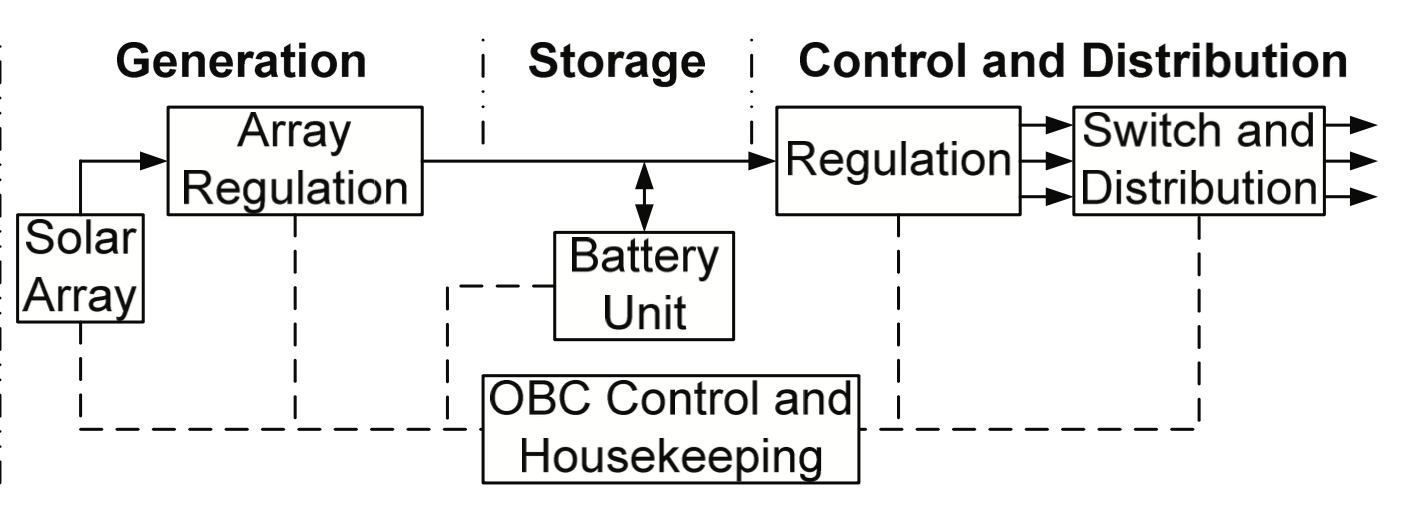
\includegraphics[scale=0.6]{./sections/SatelliteDesign/images/EPSschematics}
\centering
\caption{Basic schematics of the EPS \cite{epsbasics}}
\end{figure}

\subsubsection{Solar arrays}
The primary source of electrical power has to be photovoltaic cells, given the size of the CubeSat. 
\subsubsection{Batteries}
\subsubsection{Power management}

\subsubsection{Study of the commercial available options}
Several commercial options have to be studied.

